\section{\llm} \label{sec:method}
\begin{figure*}[t]
    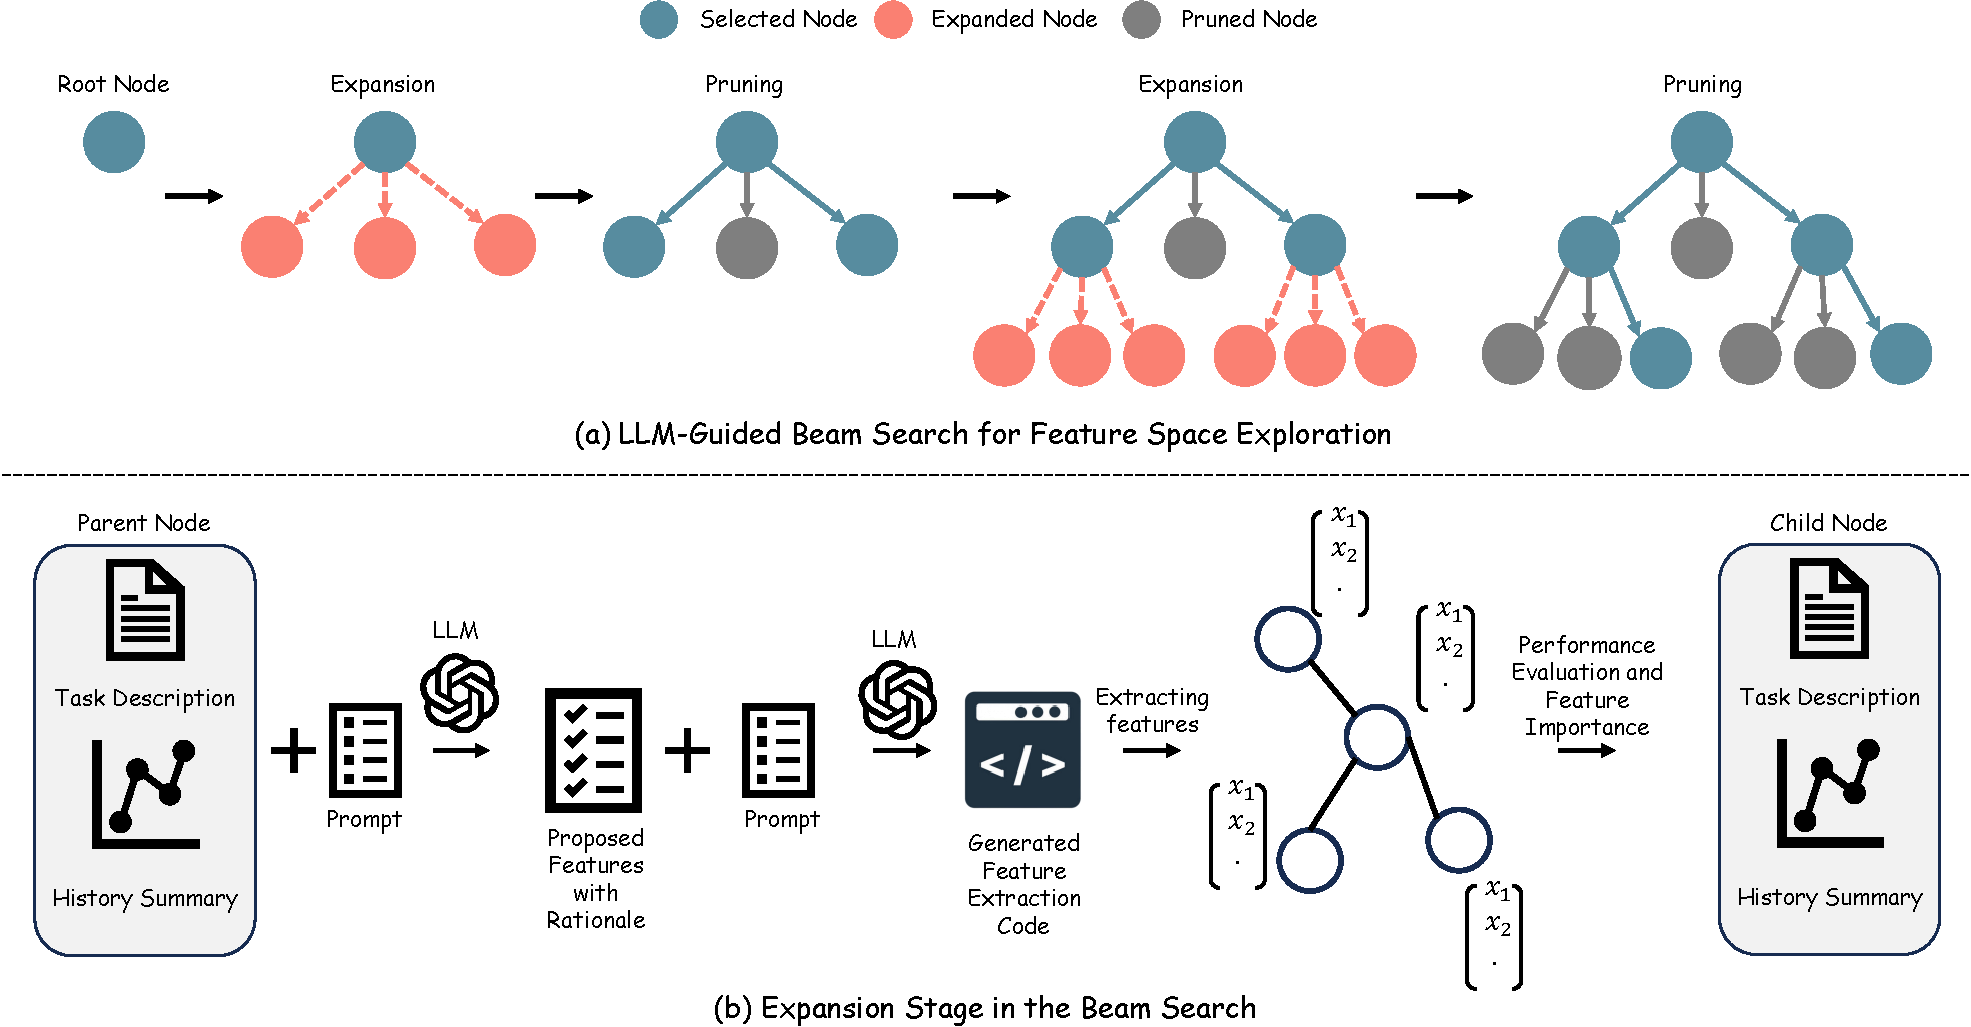
\includegraphics[width=\linewidth]{figures/LLM_cropped.pdf}
    \caption{(a) Two phases of LL2Prune, illustrated with beam width $\beta = 2$ and expansion factor $\gamma =3$. In the expansion stage, each node expands into $\gamma$ child nodes and in the pruning stage the beam grows by another depth, keeping its width size to $\beta$ after pruning out the candidate nodes with poor performances. (b) An overview of the expansion stage.  Each parent node, consisting of a task description and a history summary, is used to prompt the LLM to propose new features. A second prompt generates executable feature extraction code, which is applied to produce features. These are evaluated for performance and importance, and the resulting history is carried forward to form child nodes.}
    \label{fig:llm2prune}
\end{figure*}

The main goal of our work is to design a learning-based framework that prunes the search space through automated reasoning, making the pruning process generalize across \textcolor{black}{graph optimization problems} while accommodating additional constraints. We formalize the feature space search with LLMs as a decision tree, denoted by $\mathcal{T}$. \textcolor{black}{Each node in the tree will have its own proposed feature set and classifier, along with a running log of everything tried so far, including good features, bad features, performance results, and importance scores, so the LLM can propose new features knowing both the current state and the full path of past attempts.} Formally, each node is denoted by $n_{d,i}$, where $d \geq 0$ indicates the depth of the node in the tree and $i \in \{1, \dots, N_d\}$ indexes the node among all $N_d$ nodes at depth $d$.  

Each node $n_{d,i}$ is represented as a tuple

\[
n_{d,i} = \big(\mathcal{F}_{d,i},\mathcal{M}_{d,i}, \; g_{\theta_{d,i}}, \; \mathcal{H}_{d,i}\big),
\]
where \textcolor{black}{$\mathcal{F}_{d,i}$ is the proposed feature set, $g_{\theta_{d,i}}$ is the trained classifier on $\mathcal{F}_{d,i}$, and $\mathcal{M}_{d,i}$ denotes the performance metric of the classifier\textcolor{blue}{, defined as the combined metric $C = P_r \cdot P_g$ (see Section~\ref{sec:experiments}) evaluated on a held-out synthetic validation graph}.} The final component, $\mathcal{H}_{d,i}$, represents the history, defined as the accumulation of all feature sets, performance metrics, feature-importance vectors, and discarded features (if execution exceeds the timeout $\tau$) along the unique path from the root node $n_{0,1}$ to the node $n_{d,i}$:
\[
\mathcal{H}_{d,i} = \bigcup_{\ell=0}^{d} \; \bigcup_{j \in \pi(\ell,i)} 
\Big( \mathcal{F}_{\ell,j}, \; M_{\ell,j}, \; \text{Imp}_{\ell,j}, \; \mathcal{F}^{\text{fail}}_{\ell,j} \Big),
\]
where $\pi(\ell,i)$ denotes the ancestor index at depth $\ell$ along the path from the root to $n_{d,i}$, 
$M_{\ell,j}$ is the performance metric of the classifier, 
$\text{Imp}_{\ell,j}$ is the feature-importance vector, 
and $\mathcal{F}^{\text{fail}}_{\ell,j}$ is the set of features discarded at $n_{\ell,j}$ due to exceeding cut-off time.




% Thus, each node $n_{d,i}$ encapsulates its own feature set $\mathcal{F}_{d,i}$, trained classifier $g_{\theta_{d,i}}$, performance metric $M_{d,i}$, and feature-importance vector $\text{Imp}_{d,i}$, together with 
\textcolor{black}{The cumulative history $\mathcal{H}_{d,i}$ that records all past feature proposals, performance evaluations, and importance scores along the path from the root. This formulation ensures that the LLM generates new feature proposals with full awareness of both the local information at the node and the trajectory that led to it.} \textcolor{blue}{We condition on the full path rather than only the immediate parent because the LLM may otherwise re-propose features explored and discarded at earlier depths; providing the complete history of past attempts avoids this redundancy and reduces the number of repeated proposals during search.}







Our algorithm begins at the root node and expands the search tree one depth level at a time in a breadth-first manner. At each depth $d$, the procedure consists of two phases: \text{expansion} and \text{pruning} (as shown in Figure~\ref{fig:llm2prune}A).  



 





\textbf{Expansion.} The expansion phase of our algorithm follows the expansion step of standard beam search. Given an expansion factor $\gamma$, each node $n_{d,i}$ expands into $\gamma$ child nodes. These child nodes are produced directly by the LLM, which takes as input the task description with constraints and the accumulated history $\mathcal{H}_{d,i}$, together with a feature-generation meta-prompt $Z_{\text{feature}}$.  

This meta-prompt does not simply request new features but provides higher-level guidance on how the LLM should generate new features. Specifically, $Z_{\text{feature}}$ (see Appendix \ref{appendix:feature_generation_prompt}) instructs the LLM to enumerate and retain important features, remove redundant or uninformative ones, and propose new features derived from the current set of high-performing features. In addition, we include meta-instructions requiring the LLM to provide both a formal definition and a rationale for each proposed feature.  

% A key property of this process is that the LLM is \emph{stochastic}: even when conditioned on the same prompt and history, it can generate multiple distinct outputs. This randomness (e.g., due to temperature sampling) introduces diversity into the child nodes and enables broader exploration of the feature space. Formally, the expansion can be expressed as a stochastic mapping 


A key property of this step is that the LLM is stochastic: even under identical inputs, it can generate diverse outputs due to sampling mechanisms such as temperature, thereby broadening exploration of the feature space. Formally, the child feature sets are sampled as
\[
\big\{ \mathcal{F}_{d+1,j} \big\}_{j=1}^{\gamma}
\;\sim\;
\text{LLM}\big(Z_{\text{feature}}, \text{Task}, \text{Summary}(\mathcal{H}_{d,i})\big),
\]
where $\text{Summary}(\mathcal{H}_{d,i})$ denotes the LLM-generated summary of the history at node $n_{d,i}$. \textcolor{black}{We provide a meta-prompt $Z_{\text{summary}}$ (see Appendix \ref{appendix:summary_generation_prompt}) that summarizes the history feedback into key points and insights. Instead of providing the entire feedback history from the root to a node, this approach keeps the feedback compact and makes the reasoning process easier for the LLM to follow.} 


  

Given a child node with its generated feature set $\mathcal{F}_{d+1,j}$, we prompt the LLM with meta-prompt $Z_{code}$ (see Appendix \ref{appendix:code_generation_prompt}) to produce executable code for each proposed feature $f \in \mathcal{F}_{d+1,j}$. Executing this code yields the feature values for the training data. To ensure computational efficiency, we impose a timeout threshold $\tau$. If execution exceeds $\tau$, the failure is recorded in the history $\mathcal{H}_{d+1,j}$ and the corresponding feature is discarded. This mechanism (i) keeps the pruning process lightweight by excluding costly features and (ii) prevents further exploration of features correlated with discarded ones. If the execution of a code block raises an error, this error is passed to the LLM for the next code generation iteration.


Traditional supervised approaches \citep{lauri2023learning,tian2024combhelper} often assume that all nodes not included in the solution obtained from an exact or heuristic solver are equally unimportant, an assumption known to introduce label noise \citep{manchanda2020gcomb}. While \citet{manchanda2020gcomb} addresses this issue using a probabilistic greedy approach, where the loss of classifying each node is proportional to how frequently it is selected by solvers, we instead integrate semi-supervised learning to mitigate label noise. We then train a classifier $g_\theta$ on the features in $\mathcal{F}_{d+1,j}$. For each element $v \in \uni$, the model outputs a probability distribution $p_\theta(y \mid v)$ over labels $y \in \{0,1\}$. After a warm-up period, we retain the high-confidence nodes
\[
\mathcal{V}_{\text{conf}} = \{ v \in \mathcal{V} : \max_{y} p_\theta(y \mid v) \geq \delta \},
\]
where $\delta$ is a confidence threshold. For each $v \in \mathcal{V}_{\text{conf}}$, we assign a soft pseudo-label
\[
\tilde{y}_v = p_\theta(y \mid v).
\]
These soft pseudo-labels, together with the ground-truth labels on the supervised subset $\mathcal{V}_{\text{labeled}}$, guide further training and improve robustness by incorporating uncertainty rather than enforcing hard assignments.

\textcolor{blue}{The downstream classifier $g_\theta$ is implemented as a two-layer Graph Convolutional Network (GCN)~\citep{kipf2016semi}, operating on the LLM-proposed node-level features. For each node $v \in \mathcal{U}$, it outputs a probability $p_\theta(y=1 \mid v)$ indicating how likely the node belongs in the pruned ground set.}


\textcolor{blue}{We then validate the trained network and extract feature importance scores using an explainability algorithm, which provides insights into how different features influence the model’s predictions. This information constitutes new feedback for the corresponding child node and is appended to its history. \textcolor{blue}{To extract feature-importance vectors, we apply GNNExplainer~\citep{ying2019gnnexplainer}, which provides attribution scores indicating each feature’s contribution to the classifier’s predictions. These scores form the feedback signal $\text{Imp}_{d,i}$ used to guide subsequent feature generation.}}

% We then validate the trained network and extract feature importance scores using an explainability algorithm, which provides insights into how different features influence the model’s predictions. This information constitutes new feedback for the corresponding child node and is appended to its history. \textcolor{blue}{To extract feature-importance vectors, we apply GNNExplainer~\citep{ying2019gnnexplainer}, which provides attribution scores indicating each feature’s contribution to the classifier’s predictions. These scores form the feedback signal $\text{Imp}_{d,i}$ used to guide subsequent feature generation.}


\textbf{Pruning.} Let the set of nodes at depth $d$ be denoted by
\[
\mathcal{N}_d = \{ n_{d,1}, \dots, n_{d,N_d} \}.
\]
From this set, the algorithm maintains a beam
\[
B_d \subseteq \mathcal{N}_d, \quad |B_d| = \beta,
\]
where $\beta$ is the beam width.  During pruning, the algorithm evaluates each candidate node $n_{d+1,j} \in \mathcal{C}_{d+1}$ using its performance metric $M_{d+1,j}$, and constructs the next beam $B_{d+1}$ by selecting top-$\beta$ nodes.



The process continues until the search reaches a maximum depth $D_{\max}$, which we treat as a hyperparameter. At this point, the algorithm terminates, and the best node overall is returned as
\[
n^{\mathrm{best}} = \arg\max_{n_{d,i} \in \mathcal{T}} M_{d,i}.
\]

Finally, \textcolor{black}{when beam search finishes}, we keep only the best node found so far based on the performance metric. \textcolor{black}{In Appendix \ref{appendix:ablation}, we compare the beam-search variant against alternative configurations, e.g., a simple feedback loop and a no-feedback baseline, to isolate the effects of iterative feedback and feature-importance guidance.} \textcolor{black}{ We emphasize that \llm is a general framework that can work with any classifier and any explainability algorithms applied to that classifier.}

\textcolor{blue}{The beam search is performed once on synthetic graphs that match the structural distribution of the target domain. The metric $M$ serves as a selection criterion among candidate feature sets during search. Once the best feature set is identified, the classifier is fine-tuned on the actual target training graph and applied to prune the ground set. Algorithm \ref{alg:llm2prune} describes the full LLM2Prune pipeline.}

\begin{algorithm}[t]
\caption{\llm}
\label{alg:llm2prune}
\begin{algorithmic}[1]
\Require Task description, ground set $\mathcal{U}$, beam width $\beta$, expansion factor $\gamma$, max depth $D_{\max}$, timeout $\tau$, confidence threshold $\delta$
\Ensure Pruned ground set $\mathcal{U}' \subseteq \mathcal{U}$
\State Initialize root node $n_{0,1}$ with empty feature set and history $\mathcal{H}_{0,1} = \emptyset$
\State $B_0 \leftarrow \{n_{0,1}\}$
\For{$d = 0, 1, \dots, D_{\max} - 1$}
    \State $\mathcal{C}_{d+1} \leftarrow \emptyset$
    \For{each $n_{d,i} \in B_d$} \Comment{Expansion}
        \State $\mathrm{summary} \leftarrow \mathrm{LLM}(Z_{\mathrm{summary}},\, \mathcal{H}_{d,i})$
        \For{$j = 1, \dots, \gamma$}
            \State $\mathcal{F}_{d+1,j} \sim \mathrm{LLM}(Z_{\mathrm{feature}},\, \text{Task},\, \mathrm{summary})$
            \State Generate and execute code for each $f \in \mathcal{F}_{d+1,j}$; discard features exceeding $\tau$
            \State Train $g_{\theta_{d+1,j}}$ on $\mathcal{F}_{d+1,j}$ with semi-supervised learning (threshold $\delta$)
            \State Compute $M_{d+1,j}$ and $\mathrm{Imp}_{d+1,j}$; update $\mathcal{H}_{d+1,j}$
            \State $\mathcal{C}_{d+1} \leftarrow \mathcal{C}_{d+1} \cup \{n_{d+1,j}\}$
        \EndFor
    \EndFor
    \State $B_{d+1} \leftarrow \text{top-}\beta$ nodes in $\mathcal{C}_{d+1}$ by $M$ \Comment{Beam pruning}
\EndFor
\State $n^{\mathrm{best}} \leftarrow \arg\max_{n_{d,i} \in \mathcal{T}} M_{d,i}$
\State Fine-tune $g_{\theta^{\mathrm{best}}}$ on the target training graph
\State \Return top-ranked nodes of $\mathcal{U}$ under $g_{\theta^{\mathrm{best}}}$ as $\mathcal{U}'$
\end{algorithmic}
\end{algorithm}

% \subsection{Discussion and Practical Considerations.}





% \textbf{Why Beam Search instead of a Simple Feedback Loop?} 
% Beam search balances exploration and exploitation by retaining up to $\beta$ diverse candidates at each depth, which reduces the risk of collapsing into suboptimal regions due to noisy feedback. Compared to a simple feedback loop, our LLM-guided beam search is more stable and yields more consistent feature discovery.y.

% \textbf{Querying LLMs for Feature Search.} 
% Although querying LLMs is expensive, once a good feature set is identified for a particular problem with given constraints, the same feature set can be reused across all problems with the same constraint. We use a random graph model Homle-Kim as it closely resembles social network for feature space search and finetune the best model instance-wise training following \cite{ireland2022lense}.





 

